%%
% The BIThesis Template for Bachelor Graduation Thesis
%
% 北京理工大学毕业设计(论文)第一章节 —— 使用 XeLaTeX 编译
%
% Copyright 2020 Spencer Woo
%
% This work may be distributed and/or modified under the
% conditions of the LaTeX Project Public License, either version 1.3
% of this license or (at your option) any later version.
% The latest version of this license is in
%   http://www.latex-project.org/lppl.txt
% and version 1.3 or later is part of all distributions of LaTeX
% version 2005/12/01 or later.
%
% This work has the LPPL maintenance status `maintained'.
%
% The Current Maintainer of this work is Spencer Woo.
%
% 第一章节

\chapter{数据筛选和仓储}

\section{数据筛选}

我们的数据来自于计算机学院提供的学生数据文件,其中分为两大部分,分别是本科生信息以及研究生信息,但是其中本科生信息只包含成绩信息,而研究生信息维度较为丰富,所以使用研究生信息进行建模和推荐。其中包含2016与2017两级信息。

数据来源是教务处提供的包含学生数据的excel文件,文件共有4个,内容分别是本科生的成绩信息、研究生成绩信息、研究生学业奖学金信息以及研究生国家奖学金信息。

\subsection{本科生信息字段}

本科生成绩信息包括如下字段:

学生ID、选课课号、学年学期、课程代码、课程名称、课程性质、成绩、折算成绩、课程归属、重修标记、学分创建时间、绩点、课程属性、课程种类、考试性质、年级、学院

\subsection{研究生信息字段}

研究生成绩信息与此类似,但不同的是研究生多了一个第二课堂的excel表单,研究生与本科生信息的主要差别在于奖学金信息部分,研究生学业、国家奖学金信息均提供了8 个表单,分别是论文发表、专著论文出版、发明专利、科技获奖、科研项目、创新竞赛、荣誉称号以及其他成果,同时提供了对应每条记录的奖学金获奖情况。

研究生信息公有字段如下:

ID、学业奖学金申请等级、状态、学院培养层次、性别、民族、入学时间、学科、是否专业学位

研究生数据的论文字段如下:

论文题目、刊物会议名称、作者排序情况、论文收录情况、论文层次、中科院JCR分区大类、中科院JCR分区小类、他引情况、录用发表状态、发表时间、作者排序情况

专利字段如下:

专利名称、专利类别、专利申请号、专利申请时间、专利证书编号、专利批准日期、专利持有单位

科技获奖、创新竞赛获奖字段如下:

奖项名称、主办单位、所获奖项、获奖级别、获奖日期、奖项等级、总人数、个人排名、获奖证书编号、颁发证书单位

科研项目字段如下:

项目名称、项目类型、工作任务

出版专著字段如下:

著作名称、出版社、工作量、书号、出版日期、编著类型、作者人数、第几作者

荣誉称号/其他成果字段如下:

荣誉名称、荣誉级别、颁发单位、获得日期

在对数据进行分析之后,大致总结数据特征如下:

\section{数据库模型构建}

以数据分析为基础,这里主要对Django的数据库模式进行建构,Django是通过ORM映射对数据库进行操作,由于给定的数据源(excel文件)是关系型结构,所以我选用了关系型数据库SQLite进行数据库构建。

数据库模型构建首先需要对基础信息进行设计,基础信息按照我的构建顺序主要包括学年(期)信息、学院信息、专业信息、课程信息、学生信息。其中学年信息和学院信息是一切信息的基础,其他的信息或多或少都构建于这两个信息之上,下面对这些表中的字段与字段含义进行介绍。

\subsection{基础信息表}

\begin{enumerate}
  \item 学年(期)信息:包括学期的名称、学期起始日期、学期终止日期,通过学期信息进而转换成学年信息与数据表中的信息匹配。
  \item 学院信息:主要包括学院名称。
  \item 专业信息:包含专业名称、学生数量、学年ID、学年信息(大一、研一等)、学期信息以及学院信息,学年ID、学期信息以及学院信息是此表的外键,通过对学年信息进行筛选可以唯一的确定一条专业信息记录,虽然这张表可能存在一定冗余(专业名称、学生数量等)但是为了减少表之间取并的次数所以如此进行设计,未来可以将此表优化为拉链表节省存储空间加快检索速度。
  \item 课程信息:包括课程名称、考核方式、课程性质、学分、课程种类、学年信息等内容,主要课程的基本信息,其中有一额外生成表为lessoninfo\_affiliatedmajor,此表生成原因是一门课程可能对应于多个学院(如高数等公共基础课),而一个学院也对应多门课程,所以产生了多对多的关系,在Django中自动将此多对多关系映射为一张额外系统表,表中内容是lesson\_info 表和affiliated\_major表的主键关联信息。
  \item 学生信息:包括学生学号信息、是否为研究生、系统的登录名称、预留邮箱地址、登录密码等,学生信息与专业信息通过一额外多对多表相连,由于学生是一个实体,专业同样是一个实体,故将其之间的关系提取构建为单独关系表,在Django的代码中以through的形式表示此关系,故如下对此关系表进行解释。
  \item 关系信息表:由上文可知关系信息表是通过through代码生成,Django中关系表必须包括关联的两张表的主键作为此表外键且缺一不可,所以其中包含了学生的ID(应为对应的用户ID而非学号)以及专业信息ID,并且设置了冗余学年信息避免通过专业信息查找学年信息的连接操作提升了执行速度,同时设置关系属性字段,包括研究生、本科生等不同关系类型以及学年信息,包括研究生一年级、本科生一年级等不同信息区分,并且在最后设置起始日期与终止日期字段,使此表成为一个可通过日期查询的拉链表。
\end{enumerate}

如上是对基础信息表的介绍,接下来是对学生部分的个人信息表进行构造。

\subsection{个人信息表}

个人信息表共包括8部分内容,其中有7个表是从所给数据文件中直接得到,分别是论文发表、专著论文出版、发明专利、科技获奖/创新竞赛、科研项目以及荣誉称号/其他成果,同时包括一个存储了学生奖学金获奖历史表,论文发表等表字段内容与excel所给字段内容一致不再赘述,值得注意的是有些空字段需要额外处理才能向数据库中录入内容,除此以外科技获奖、创新竞赛的表以及荣誉称号、其他成果表的字段内容基本一致,所以通过一个类型字段进行区分即可省略一张表,同时学生与奖学金信息同样构成了一个关系即为学生的奖学金获奖历史,这个表同样可以看作多对多关系生成的一个表,所以会额外生成一张带有学生ID和奖学金ID作为外键的表。

\subsection{奖学金表}

接下来是奖学金表的构造,因为之前考虑将系统设计为B/S架构,所以需要设计带有奖学金信息的推送网页内容,故设计奖学金信息表、奖学金信息分级表、奖学金网页内容表,这其中奖学金信息表主要包含奖学金的名称、奖励金额等,同时未来还可扩充额外要求字段。奖学金信息分类表主要是由于某个类型的奖学金可能有多个分级,需要对不同的分级进行考虑,此表能够减少冗余,并且在推送内容填充URL的时候可以直接根据奖学金是否有分级填充不同的URL提高奖学金在网页推送部分的效率,除此以外还可以增加数据库的层次化结构。同时表中的推送内容使用Markdown格式,方便如Ueditor等富文本编辑器进行编辑。同时可以使用Python 的word2md包的Markdown转换工具将word文件上传自动转为Markdown方便在线编辑使用。

\section{数据导入与数据库填充}

向数据库中填充数据使用的是Django自带的ORM映射,通过调用接口而非注入SQL命令实现更安全的数据操作方式,所有与数据填充有关的代码均在utils中,其中首先需要调用os.environ.setdefault命令读取Django启动配置,然后使用django.setup()命令实现Django的初始化,Django启动后可以通过引入不同的model对模型直接进行操作,同时还使用了python的xlrd包对excel文件进行读取。

数据库填充首先填充的是学年、学院、专业、课程以及学生信息,在填充学生个人的时候使用集合对所有数据表中的学生ID进行去重统计,除此以外还需要注意对某些特殊字段进行处理,包括对空字段进行填充等。由于在不同apps的model中设置好了部分分类字段的映射(分类字段是以CharField的形式进行保存,用元组设置了映射规则),所以需要用字典对文本进行处理与转换,最终在数据库中保存缩写后的元素。

\section{数据库信息统计与E-R图}

以下是对导入内容进行统计:
\newpage

\begin{table}[htbp]
  \linespread{1.5}\zihao{5}\centering\caption{数据库内容统计}\label{数据内容统计}
  \begin{tabular}{*{5}{>{\centering\arraybackslash}p{2cm}}}
    \hline
        & 总人数    & 获奖人数  & 奖项个数 &  奖项个数>10\\ \hline
    研究生信息  & 1469 & 186 & 9 &  4\\
    本科生信息 & 1441  & 无  & 无  & 无   \\ \hline
    \end{tabular}
\end{table}

可以看到只有研究生有获奖信息,而其中可供聚类的label不超过4个。

如图\ref{E-R-image}是数据库的E-R图:

\begin{figure}[htb]
  \vspace{13pt} % 调整图片与上文的垂直距离
  \centering
  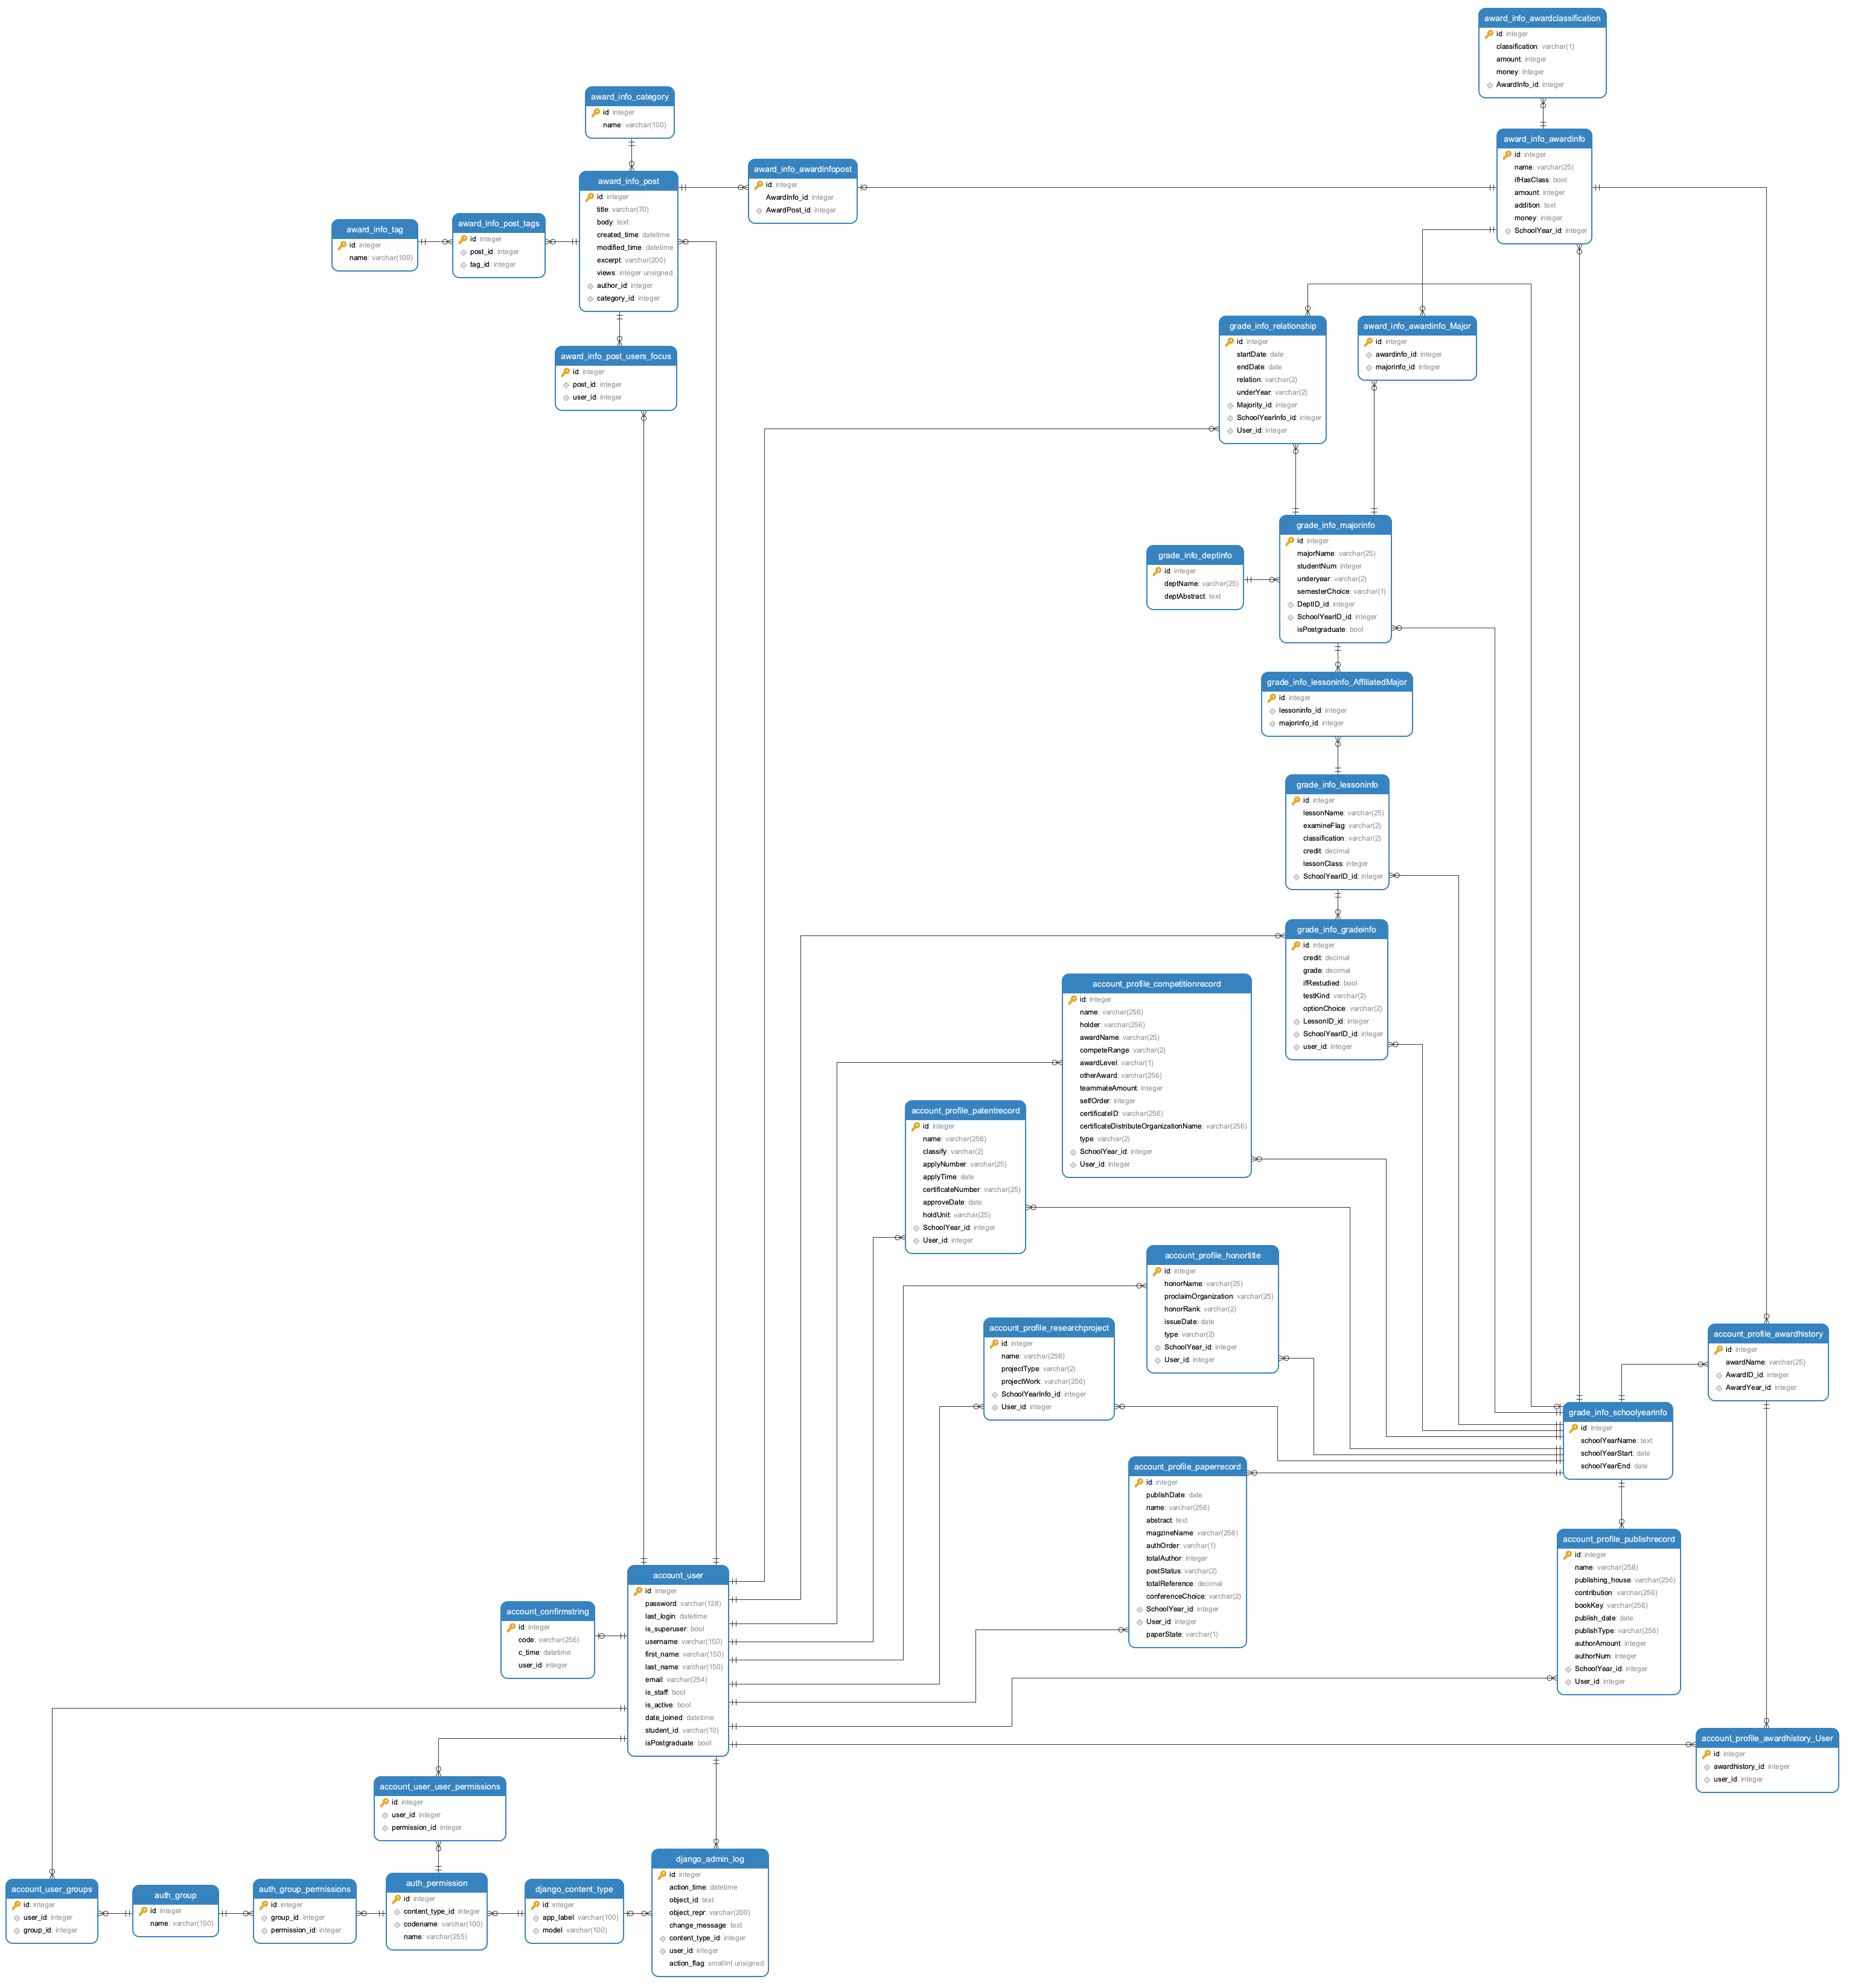
\includegraphics[width=0.7\textwidth]{images/database-ER.png}
  \caption{数据库E-R图}\label{E-R-image} % label 用来在文中索引
\end{figure}
